
\documentclass[x11names,svgnames,aspectratio=169]{beamer}

\usetheme{metropolis}
\setbeamertemplate{caption}{\raggedright\insertcaption\par}
\setbeamercolor{block title}{fg=LightSkyBlue4}
\newenvironment<>{importantblock}[1]{%
  \begin{actionenv}#2%
    \def\insertblocktitle{#1}%
    \par%
    \mode<presentation>{%
      \setbeamercolor{block title}{%
        use=normal text,
        fg=normal text.fg,
        bg=normal text.bg!80!fg
      }
      \setbeamercolor{block body}{
        use={block title, normal text},
        bg=block title.bg!50!normal text.bg
      }
    }%
    \usebeamertemplate{block begin}}
  {\par\usebeamertemplate{block end}\end{actionenv}}
\newenvironment<>{decisionblock}[1][Statement of the problem]{%
  \begin{actionenv}#2%
    \def\insertblocktitle{#1}%
    \par%
    \mode<presentation>{%
      \setbeamercolor{block title}{%
        use=normal text,
        fg=normal text.fg,
        bg=normal text.bg!80!fg
      }
      \setbeamercolor{block body}{
        use={block title, normal text},
        bg=block title.bg!50!normal text.bg
      }
    }%
    \usebeamertemplate{block begin}}
  {\par\usebeamertemplate{block end}\end{actionenv}}
\usepackage{fontspec}
\usepackage[french, frenchkw]{algorithm2e}
\SetKwFor{Pc}{Pour chaque}{faire}{fin}
\SetKwProg{Fn}{Fonction}{:}{}
\usepackage{textcomp}
\usepackage{minted}
\usepackage[framemethod=TikZ]{mdframed}
\usepackage{pdfpages}
\usepackage{qrcode}
\usepackage[francais]{babel}
\usepackage{xspace}
\usepackage[normalem]{ulem}
\usepackage[backend=biber,style=authoryear,url=false]{biblatex}
\addbibresource{Bibliography.bib} % Bibliography file
\usepackage{amsmath}
\usepackage{mathtools}
\usepackage{pifont}% http://ctan.org/pkg/pifont
\newcommand{\cmark}{\ding{51}}%
\newcommand{\xmark}{\ding{55}}%
\usepackage{marvosym}
\usepackage{tikz}
\usetikzlibrary{calc, positioning, arrows, automata, fadings, decorations.pathmorphing, shapes, patterns, tikzmark, fit, chains, snakes, shapes.multipart}
% https://tex.stackexchange.com/questions/401884/how-do-i-change-hyperlinks-color-only
\hypersetup{
  colorlinks,
  allcolors=.,
  urlcolor=DarkBlue,
}


\author{}
\date{Lundi 21 octobre 2024}

\title{
\includegraphics[width=0.75\textwidth]{../../img/logo-igm.png} \\ Algorithmique et Programmation 1}
\institute{L1 Mathématiques - L1 Informatique \\ Semestre 1}

\begin{document}

\maketitle

\begin{frame}{CC1 : Comment et quoi ?}
  \begin{block}{Horaire}
    \vspace{0pt}
    \textbf{Lundi 4 novembre 13h-15h} (tiers-temps : 15h40) en A1, A2, A5
  \end{block}
  \pause
  \begin{block}{Contenu}
    \vspace{-0.25em}
    \begin{itemize}
    \item Tout ce qu'on a vu, y compris les séances de cette semaine
    \item Les slides \alert{et} les notes de cours
    \item QCM
    \item Questions de programmation écrites
    \item Mini-problème
    \end{itemize}
  \end{block}
  \pause
  \begin{block}{Sur la triche}
    \vspace{-0.25em}
    \begin{itemize}
    \item L'examen est \textbf{individuel}
    \item Tolérance zéro
    \end{itemize}
  \end{block}
\end{frame}

\begin{frame}{Questions ouvertes et mini-problème}
  Voir \href{DOC-catalog.pdf}{le sujet de l'an dernier}
\end{frame}


\section{Approfondissements : les listes \newline (de listes (de listes (\dots)))}

\begin{frame}{Revenons à notre morpion}

  
\includegraphics[width=\textwidth]{slide_morpion.png}
  \end{frame}

\begin{frame}{Revenons à notre morpion}

  Démo sur Thonny

  \pause

  \begin{block}{Les leçons à en tirer}
  \begin{itemize}
    \item Une liste de listes se comporte comme une matrice : \mintinline{python}{grille[i][j]} permet d'accéder à la case $(i, j)$ \newline (et la modifier)
    \item Lorsqu'on utilise plusieurs fois une liste, c'est la \alert{même} liste même si on a l'impression de l'avoir copiée
    \item Factoriser le code en fonctions permet de le rendre plus lisible
    \item Ces fonctions peuvent \alert{modifier} la liste donnée en argument
  \end{itemize}
  \end{block}
\end{frame}

\begin{frame}[fragile]{La liste de listes comme matrice}

  \begin{mdframed}[roundcorner=5pt]
\begin{minted}{python}
grille = [
  #   0    1    2
    ["a", "b", "c"], # 0
    ["d", "e", "f"], # 1
    ["g", "h", "i"]  # 2
]
\end{minted}
\end{mdframed}

\begin{block}{Accéder à une ligne et à une case}
  \begin{columns}
    \begin{column}{0.5\textwidth}
  \begin{mdframed}[roundcorner=5pt]
  \begin{minted}{python}
l = grille[1]
>>> ["d", "e", "f"]
l[2]
>>> "f"
\end{minted}
\end{mdframed}
\end{column}
    \begin{column}{0.5\textwidth}
  \begin{mdframed}[roundcorner=5pt]
  \begin{minted}{python}
(grille[1])[2]
>>> "f"
grille[1][2]
>>> "f"
    \end{minted}
    \end{mdframed}
\end{column}
\end{columns}
\end{block}

\end{frame}

\begin{frame}[fragile]{La liste de listes comme matrice}

  \begin{mdframed}[roundcorner=5pt]
\begin{minted}{python}
grille = [
  #   0    1    2
    ["a", "b", "c"], # 0
    ["d", "e", "f"], # 1
    ["g", "h", "i"]  # 2
]
\end{minted}
\end{mdframed}
\begin{block}{Modifier une case}
  \begin{mdframed}[roundcorner=5pt]
  \begin{minted}{python}
l = grille[1]
>>> ["d", "e", "f"]
l[2] = "j"
print(grille)
>>> [['a', 'b', 'c'], ['d', 'e', 'j'], ['g', 'h', 'i']]
\end{minted}
\end{mdframed}
\end{block}
\end{frame}

\begin{frame}[fragile]{La liste de listes comme matrice}

  \begin{mdframed}[roundcorner=5pt]
\begin{minted}{python}
grille = [
  #   0    1    2
    ["a", "b", "c"], # 0
    ["d", "e", "j"], # 1
    ["g", "h", "i"]  # 2
]
\end{minted}
\end{mdframed}
\begin{block}{Modifier une case (suite)}
  \begin{mdframed}[roundcorner=5pt]
  \begin{minted}{python}
(grille[2])[2] = "k"
print(grille)
>>> [['a', 'b', 'c'], ['d', 'e', 'j'], ['g', 'h', 'k']]
grille[0][1] = "l"
>>> [['a', 'l', 'c'], ['d', 'e', 'j'], ['g', 'h', 'k']]
    \end{minted}
    \end{mdframed}
\end{block}
\end{frame}

\begin{frame}[fragile]{La copie superficielle}

  \begin{mdframed}[roundcorner=5pt]
\begin{minted}{python}
ligne = ["a", "b", "c"]
grille = [ligne, ligne, ligne]
print(grille)
>>> [["a", "b", "c"], ["a", "b", "c"], ["a", "b", "c"]]
\end{minted}
\end{mdframed}
\begin{block}{Modifier une (des ?) case}
  \begin{mdframed}[roundcorner=5pt]
  \begin{minted}[escapeinside=||]{python}
ligne[1] = "d"
print(grille)
|\pause|>>> [['a', 'd', 'c'], ['a', 'd', 'c'], ['a', 'd', 'c']]
|\pause|grille[0][2] = "e"
|\pause|>>> [['a', 'd', 'e'], ['a', 'd', 'e'], ['a', 'd', 'e']]
    \end{minted}
    \end{mdframed}
\end{block}
La preuve sur \href{https://pythontutor.com/}{Python Tutor}.
\end{frame}

\section{Les fonctions sur les listes}

\begin{frame}[fragile]{Mutabilité, immutabilité}

  \begin{block}{Rappel}
    \vspace{0pt}
  Une fonction \alert{ne peut pas modifier}\footnote{\onslide<2>{Sauf en utilisant les mots-clés \mintinline{python}{global} et \mintinline{python}{nonlocal}, mais ne faites pas ça svp.}} une variable de type \mintinline{python}{int} donnée en argument :
\vspace{-0.5em}
  \begin{mdframed}[roundcorner=5pt]
  \begin{minted}{python}
def essaie_de_modifier_pour_voir(x):
    x = 5

x = 12
essaie_de_modifier_pour_voir(x)
print(x)
>>> 12
\end{minted}
\end{mdframed}

\vspace{-0.5em}
C'est aussi vrai pour tous les types ``primitifs'' : \newline \mintinline{python}{int}, \mintinline{python}{float}, \mintinline{python}{str}, \mintinline{python}{bool}.

\vspace{-0.5em}
On dit que les types primitifs sont \alert{immutables}.
\vspace{1em}
  \end{block}

  \end{frame}

\begin{frame}[fragile]{Mutabilité, immutabilité}
  Une fonction \alert{peut modifier} la liste donnée en argument :
  \begin{mdframed}[roundcorner=5pt]
  \begin{minted}{python}
def essaie_de_modifier_pour_voir_liste(lst):
    lst[0] = 5

lst = [12]
essaie_de_modifier_pour_voir_liste(lst)
print(lst)
>>> [5]
\end{minted}
\end{mdframed}

On dit que les listes sont \alert{mutables}.
  \end{frame}

  \section{Les itérables}

\begin{frame}{Les itérables}

  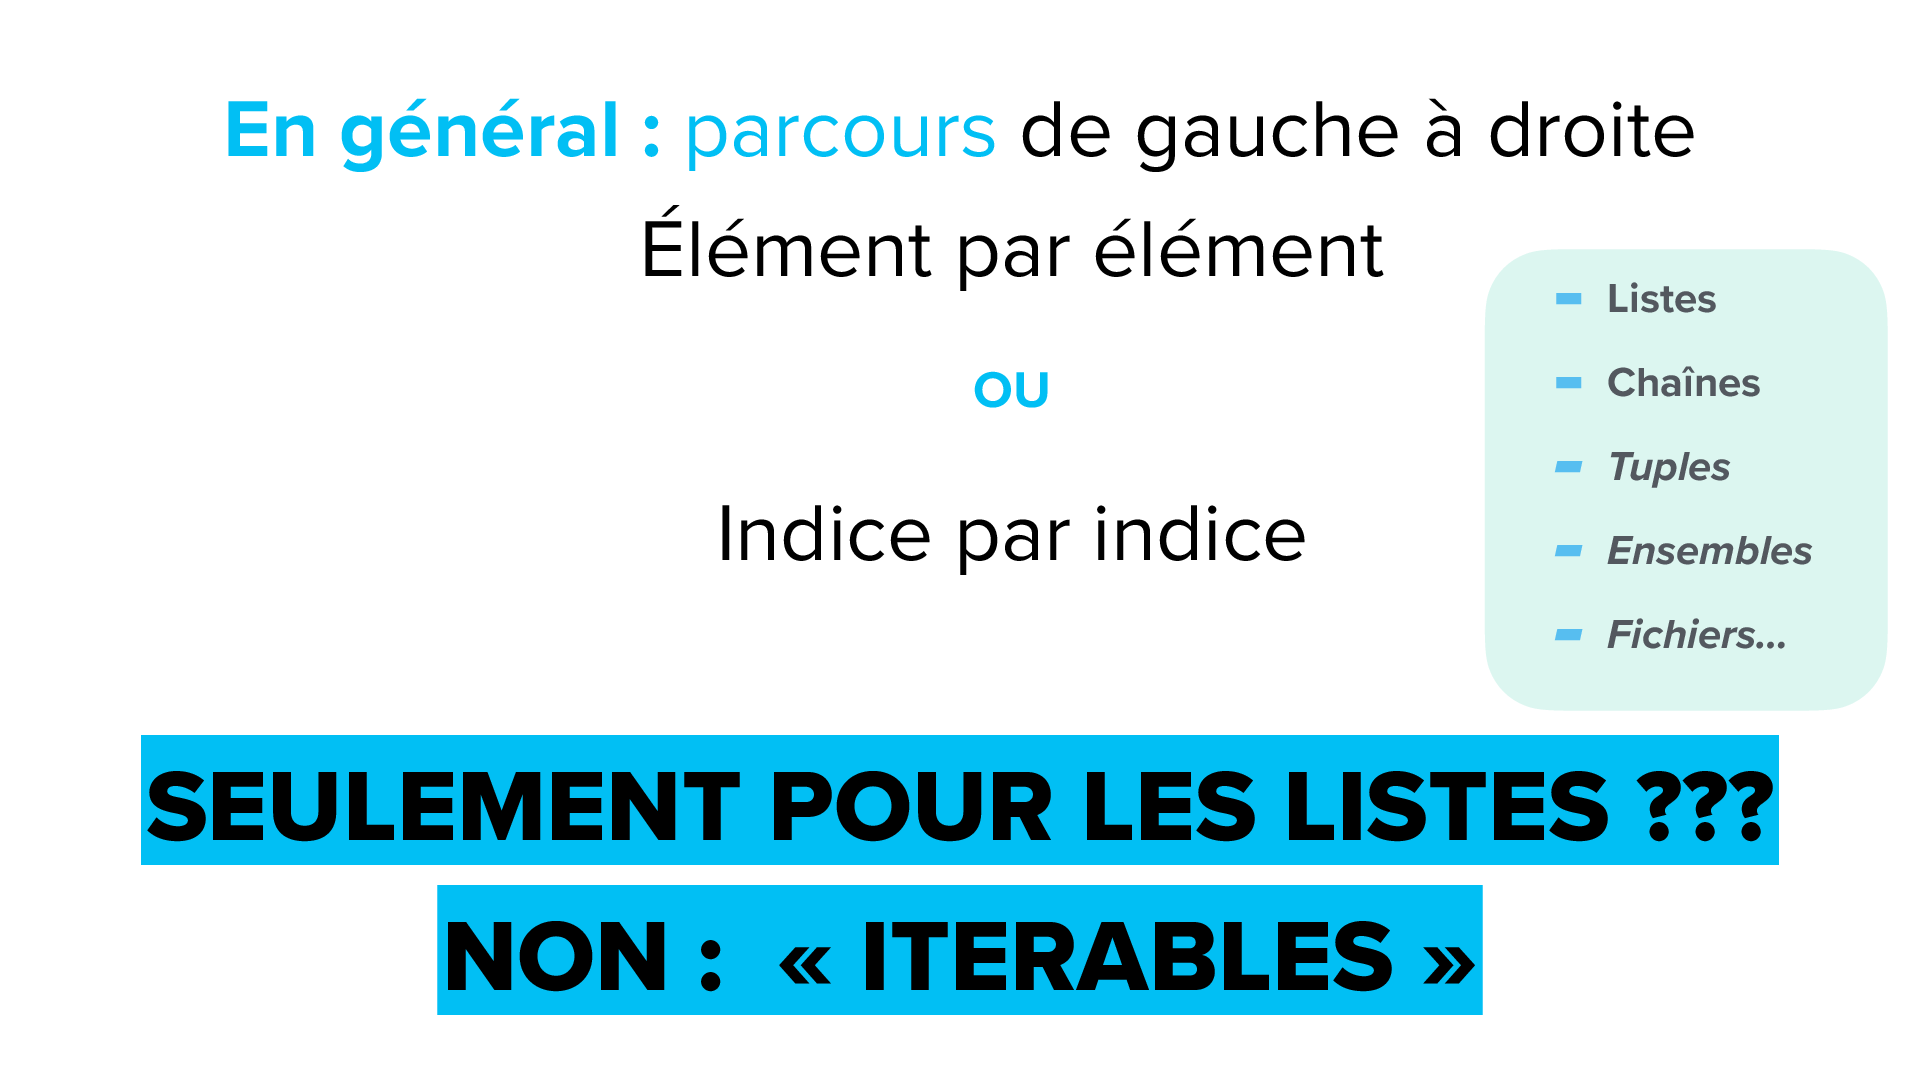
\includegraphics[width=\textwidth]{slide_iterables.png}
  \end{frame}

\end{document}



%%% Local Variables:
%%% TeX-engine: xetex
%%% TeX-command-extra-options: "-shell-escape"
%%% End:
